\subsection{Data Processing and Mixed Precision Training}
\label{back:data}

\subsubsection{Data Normalization}

Normalization is a technique of which data is transformed from it's original scale, to a more standard scale \cite{ali2014data}. These techniques are normally used when the dataset has elements of different ranges. Normalization can contribute to faster convergence, and it's why they are as commonly used when preprocessing data. 

\textbf{MinMax Normalization} 

This algorithm transforms data to a specified range, most often $[0, 1]$ but it can also be $[-1, 1]$ or any other range.
Minmax normalization can be described as follows:

\begin{equation}
   x_{\text{normalized}} = \dfrac{x - x_{min}}{x_{max}-x_{min}}
\end{equation}
\vspace{0.2cm}

where $x$ denotes the data, $x_{min}$ and $x_{max}$ is the minimum and maximum in $x$. \\

\subsubsection{Half Precision Training}

Working with large datasets and \acrshort{dnn}s can be rather time- and resource consumptive. To address this, one can cast the datatype from single precision to half precision, along with weights, biases and losses. This will reduce loss of accuracy and information, but it can drastically lower memory consumption and decrease training time. It is important to note that casting of data occurs with normalization techniques, the order of which operation happens first is quintessential. If the data is casted to half precision before normalization, the normalization will be based on a slightly inaccurate representation of the data, but the computation of the normalized data will be faster. If normalization were to occur first, less detail about the data would be lost, but at the expense of being more computational intensive. \\

\textbf{Mixed precision training}

Mixed precision training, introduced in 2018 \cite{micikevicius2018mixed}, is a technique where the weights, activations and biases of a neural network is stored in single precision, while the data itself stays in it's original format. It allows for reduced memory consumption, while also speeding up operations of deep neural nets. Additionally, the amount of $\si{\kilo\watt\hour}$ required to train the neural nets would decrease, thus reducing both the cost and the environmental tax by training neural nets. This becomes more important the larger the datasets, models and the sheer amount of GPUS required to train massive workloads. This introduce the concept of loss scaling, where the losses needs to be adjusted based on the weights. \\

\mycomment{
\subsection{Dataloaders}

If the datasets contain information about the data and how to retrieve a single instance, the dataloaders job is to create an object that can be iterated over, containing $n$ amount of batches, and transferring these data to the wanted devices. In the case of data parallel multi-gpu training, when the data is loaded, it's \textit{sharded} across the different gpus, in a manner that balances the load of each gpu. Let's say we have a batch  of size $[4, 5, 5]$ and we have two gpus available. The dataloader can split this Tensor in two batches, where each of the gpus get a tensor of size $[2, 5, 5]$. By sharding the data along the first axis, ideally we can half the amount it takes, not taking data transfer time into consideration. 

\begin{figure}[!h]
    \centering
    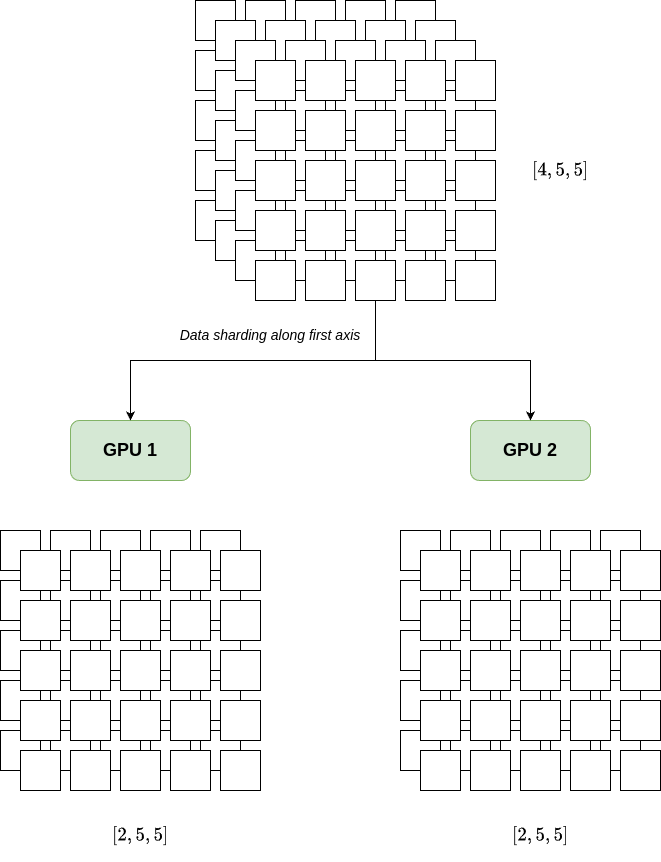
\includegraphics[scale=0.4]{figures/sharding.png}
    \caption{Example of data sharding with 2 gpus, and a original Tensor of size [4,5,5]}
    \label{fig:sharding}
\end{figure}


\textbf{Parallel loading}

When iterating over a dataloader, each element of the batch is retrieved and undergoes transformations. Depending on the batch size and  the size of the data, this procedure can be very resource-intensive and time-consuming. To mitigate this, we can introduce the concept of parallel batch loading. Instead of gathering and transforming the data sequentially, one can leverage available resources to do this operation in a parallel manner. Algorithm \ref{alg:parallel-batch-loading} details how such an operation is conducted.


\begin{algorithm}
\caption{Parallel Batch Data Loading}\label{alg:parallel-batch-loading}
\begin{algorithmic}
\Require BatchIndices, N
\Ensure BatchData, LoadSingleData
\State Initialize empty list BatchData
\State Create ThreadPool with N threads
\For{each Index in BatchIndices}
    \State Submit LoadSingleData(Index) to executor
\EndFor
\For{each completed Future from executor}
    \State Data $\gets$ Future.result()
    \State Append Data to BatchData
\EndFor
\State \Return BatchData
\end{algorithmic}
\end{algorithm}
}

\subsubsection{Overfitting and Early Stopping}

Overfitting is a common problem within \acrlong{ml} \cite{srivastava2014dropout}. It occurs when a model is trained , and fails to fit additional data. In addition to popular techniques such as dropout \cite{srivastava2014dropout}, \textit{early stopping} is a regularization technique that aims to avoid overfitting. When training an optimizer such as \acrshort{adam} \cite{kingma2017adam}, or \acrshort{sgd} \cite{Rumelhart1986, Bottou2012}, one can notice when a model is overfitting by studying the validation loss. If the validation loss $L_v$ starts increasing, the early stop mechanism will stop the training altogether if no improvement of $L_v$ is found after $p$ number of epochs. A formal definition can be given as such:

\begin{align*}
&\text{Stop at epoch } T \text{ if:} \\
&\forall i \in \{T-p+1, ..., T\}: L_v(i) > L_v^* - \epsilon \\
&\text{where } L_v^* = \min_{j=1}^{T} L_v(j) \\
\\
&\text{Given:} \\
&L_v(t) \text{ is the validation loss at epoch } t \\
&p \text{ is the patience (number of epochs to wait)} \\
&\epsilon \text{ is a small threshold for improvement}
\end{align*}

\subsubsection{Parallelism within \acrlong{ml}}

With rapid evolving deep learning architectures, the importance of scalable model training and networks grows larger each year. It is even estimated that these networks grow 1,5x each year \cite{9499913}, making parallelization a vital topic when it comes to \acrlong{ml} to accommodate ever increasing memory needs. Several different hardware accelerators have been created to best accommodate these needs, the most apparent of these are \acrshort{gpu}s. NVIDIA have for several years dominated this market, and their hardware is becoming faster and increasing in memory. \\

By workers, we mainly refer to \acrshort{gpu}s, but this could also be processors or other types of hardware accelerators such as TPUs.


\subsubsection{Model Parallelism}

\acrshort{dl} models need to store a lot of data. Weights and biases tend to take up a lot of memory, thus requiring the need of splitting up a model across several workers. As an example, given a model $M$ of 50 layers, we can split this model in 2 parts by having a worker $A$ manage the first 25 layers, and worker $B$ manage the latter half.
The overhead of transferring data across these workers can become a bottleneck, so this should only be utilized when absolutely necessary.

\subsubsection{Data Parallelism}

Data parallelism refers to partitioning data across multiple workers. Given a dataset $X$, we can split $X$ across the workers and store a copy of the model $M$ on each worker, calculate gradients across them all and update the trainable parameters for $M$. 

\subsubsection{Hybrid Parallelism}

This kind of parallelization combines the two previously mentioned techniques. First, $M$ is split across several workers, and then $X$ is subsequently split across multiple workers. 